\documentclass[12pt,a4paper]{article}
\usepackage{appendix}
\usepackage[utf8]{inputenc}
\usepackage[french]{babel}
\usepackage[T1]{fontenc}
\usepackage{amsmath}
\usepackage{amsfonts}
\usepackage{amssymb}
\usepackage{graphicx}
\usepackage[left=2cm,right=2cm,top=2cm,bottom=2cm]{geometry}
\author{Javaid Mohammad-Habib, Carbonneau Danaël}

\usepackage[Glenn]{fncychap}

\usepackage{fancybox}

\usepackage{multicol}
\usepackage[hidelinks]{hyperref}

\usepackage{xcolor}
\usepackage{listings}
\lstset{numbers=left, 
		stepnumber=1,
		breaklines=true,
		numberstyle=\footnotesize,
		captionpos=b,
		}

\newcommand{\pythonstyle}{\lstset{
		language=python,
		basicstyle=\ttfamily ,
		keywordstyle=\bfseries\color{blue},
		commentstyle=\itshape\color{green}}
}
\newcommand{\maclestyle}{\lstset{
		language=caml,
		basicstyle=\ttfamily ,
		keywordstyle=\bfseries\color{blue},
		commentstyle=\itshape\color{green},
		otherkeywords={reg,default,exec}}
}
		
\newcommand{\cstyle}{\lstset{
		language=C,
		basicstyle=\ttfamily,
		keywordstyle=\bfseries\color{blue},
		commentstyle=\itshape\color{green}}
}

\newcommand{\verilogstyle}{\lstset{
		language=Verilog,
		basicstyle=\ttfamily,
		keywordstyle=\bfseries\color{blue},
		commentstyle=\itshape\color{green}}
}

\newcommand{\vhdlstyle}{\lstset{
		language=VHDL,
		basicstyle=\ttfamily,
		keywordstyle=\bfseries\color{blue},
		commentstyle=\itshape\color{green}}
}
\begin{document}


\begin{titlepage}
\newcommand{\HRule}{\rule{\linewidth}{0.5mm}}



\center 
\bigskip
\textsc{\LARGE
Sorbonne Université
}
 \\[4cm]
 \HRule \\[0.4cm]
{ \huge \bfseries Devoir de Programmation \\[0.15cm] }

\HRule \\[2cm]

\begin{large}
Danaël CARBONNEAU (28709878), Javaid Mohammad-Habib (21307723) \\
\end{large}

\begin{huge}
Diagrammes de décision binaires (\textit{ZDD}).
\end{huge}

\vfill

Master STL, Semestre 1, septembre - janvier 2023 - 2024 \\ [1cm]

\end{titlepage}



\tableofcontents



\section{Échauffement}

Le code associé à cette partie se trouve dans le fichier \textit{echauffement.ml}. 

Nous représenterons dans la suite du projet les entiers précis par ce type : \texttt{type entier\_precis = int64 list;;}. Nous avons également écrit pour les manipuler une primitive permettant l'ajout en fin, une permettant de récupérer la tête, et une permettant de récupérer sa suite.

Par la suite, nous avons pu écrire les fonction nous permettant de manipuler les grands entier sous plusieurs représentations (listes d'entiers 64 bits, listes de booléens). Grâce aux fonctions \texttt{Int64.unsigned\_rem} \texttt{Int64.shitf\_right\_logical}, et \texttt{Int64.shift\_left}, on traite bien notre entier comme s'il n'était pas signé, donc en utilisant ses 64 bits.

Concernant la génération aléatoire, depuis la version \href{4.14}{https://ocaml.org/releases/4.14.0}, le module Random implémente une fonction \texttt{Random.bits64()} qui nous retourne 64 bits aléatoires représentés sur un entier 64 bits. Lorsqu'on teste \texttt{GenAlea}, on voit alors bien des nombres négatifs apparaître dans la décomposition (c'est à dire des nombres ayant leur bit de poids fort à 1, ce qui correspond à ce qu'on veut pour traiter les entiers 64 bits de la liste comme des bitmaps). Il est donc nécessaire d'avoir cette version d'installée.
%TODO : annexe howto installer ocaml 4.14.1


\section{Arbres de Décision}
Le code associé à cette partie se trouve dans le fichier \textit{Arbre\_decision.ml}.

La structure est faite à l'aide d'un type Somme (et d'un alias de type pour la profondeur) :

\medskip
\texttt{type profondeur = int}

 \texttt{type arbre\_decision = Feuille of boolean \\
 | Noeud of profondeur* arbre\_decision * arbre\_decision}.

\medskip


\section{Compression de l’arbre de décision et ZDD}

Le code associé à cette partie se trouve dans les fichiers \textit{deja\_vus.ml}, \textit{compression.ml}, et \textit{dot.ml}.

\subsection{Choix d'implémentation : l'utilisation de foncteurs}

L'algorithme de compression utilise une structure permettant de conserver une trace des grands entiers déjà vus. Étant donné que nous serons amenés à utiliser cette algorithme avec deux structures (une liste dans cette partie, une arborescence dans la suivante), nous avons décidé d'utiliser le mécanisme de \textbf{foncteurs} offertes par le langage OCaml.

En effet, du point de vue de l'algorithme, il nous faut une structure qui nous rend trois services : 

\begin{itemize}
\item créer une structure vide
\item insérer un couple (grand entier, arbre de décision) dans la structure
\item déterminer si un grand entier est dans la structure (auquel cas, retourner l'arbre de décision associé, rien sinon).
\end{itemize}

On va donc définir un type de modules correspondant à cette interface : il s'agit du module \texttt{SetDejaVus}, dont la signature est donnée dans \textit{deja\_vus.ml}.

De là, on veut pouvoir utiliser n'importe quelle structure pour laquelle seraient définis ces trois services dans notre algorithme. Pour cela, on va écrire, dans \textit{compression.ml} un foncteur \texttt{AlgoCompression}, c'est à dire un module paramétré par le type de modules \texttt{SetDejaVus}. À l'intérieur de ce foncteur, on peut désormais écrire notre fonction de compression, qui utilise le module passé en paramètres pour avoir :
\begin{itemize}
\item Le type de la structure utilisée
\item Les opérations, qui sont nécessaires à l'algorithme, dont l'implémentation va dépendre de la structure
\end{itemize}


On arrive ainsi à factoriser notre code et séparer le déroulement de l'algorithme de la gestion sous-jacente, de notre ensemble d'arbres déjà vus.

\subsection{Manipulation des arbres de compression}

Dans l'algorithme de compression, nous voulons remplacer, lorsqu'une règle de compression est appliquée, le noeud courant N par un autre noeud vis à vis de son père. Étant donné que notre fonction reconstruit l'arbre compressé en fonction des appels récursifs, il nous suffit pour cela de retourner le bon nœud remplaçant le nœud N par celui qui lui correspond dans notre arbre compressé.

La représentation des valeurs, et notamment des types sommes, nous permet de ne pas avoir besoin d'utiliser de références : les valeurs en OCaml sont soit des entiers, soit des pointeurs vers un bloc sur le tas. Lorsqu'on ajoute un noeud en tête de notre ensemble de (grand entier, noeud) déjà visités, on créé sur le tas un bloc contenant un pointeur vers notre noeud, et un pointeur vers la suite de la liste. Lorsqu'on le récupère ailleurs dans le code, on ne récupère alors pas de copie mais bien un pointeur vers le nœud souhaité. 


\subsection{Faire des graphiques avec le langage dot}

Dans le fichier \textit{dot.ml}, nous avons écrit deux fonctions : une qui parcourt l'arbre de décision pour écrire dans un fichier ce qu'il faut pour chaque nœud, et une qui s'occupe de formater comme souhaité chaque noeud.

\subsubsection{Formattage en dot}

Dot nous permet de faire des graphes en décrivant les arrêtes, et potentiellement les nœuds, en les écrivant lignes après lignes. Il nous faut donc, pour transcrire facilement notre graphe, un identifiant unique par nœud (qui ne sera pas affiché, grâce aux labels). On peut ensuite, pour chaque nœud interne du graphe, écrire dans notre fichier la mise en forme correspondante : 

\begin{description}
\item[Noeud interne]  : \texttt{idN [label = profondeur];
 idN -> idFG [style=dotted]; 
 idN -> idFD [style=dotted];}
 
 \item [Feuille] :\texttt{idN [label = True|False]}
\end{description}


\subsubsection{Des identifiants uniques... avec un peut de magie}
Afin d'avoir un \textbf{idN unique}, nous avons choisi d'utiliser la fonction \texttt{Obj.magic}. Il s'agit d'une fonction (\textit{peu recommandée}) de la librairie standard OCaml : elle force un cast de type sur l'objet qu'elle manipule (soit un entier, soit un bloc, donc un pointeurs vers le tas), qui est dans tous les cas codé sur un entier (soit de taille 32bits, doit de taille 64), et retourne sa valeur "réelle" (au runtime). 

Étant donné que nous appliquons cette fonctions à des arbres de décision, c'est à dire un type somme, c'est une manière de récupérer l'adresse de chaque block. Il s'agit donc d'un nombre \textbf{unique} à chaque nœud dans notre arbre, ce qui en fait un candidat parfait pour notre identifiant\footnote{Le système d'identifiant par pointeur nous permet également de vérifier que la compression s'est aussi faite en mémoire.}.


\subsubsection{Résultats}

Nous avons alors pu obtenir un affichage graphique de l'arbre de l'énoncé avant et après compression. 


\begin{figure}[hbtp]
\centering
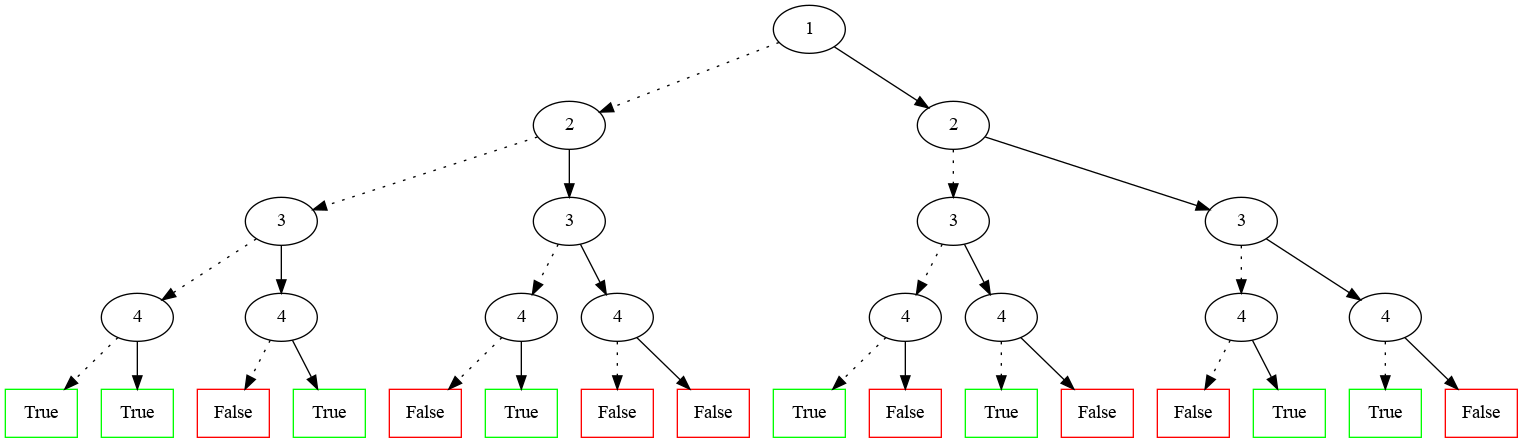
\includegraphics[scale=0.3]{../Images/arbre_non_compresse.png} 
\caption{Arbre de décision issu de la table de vérité de taille 16 construite sur le grand entier [25899]}
\end{figure}



\begin{figure}[hbtp]
\centering
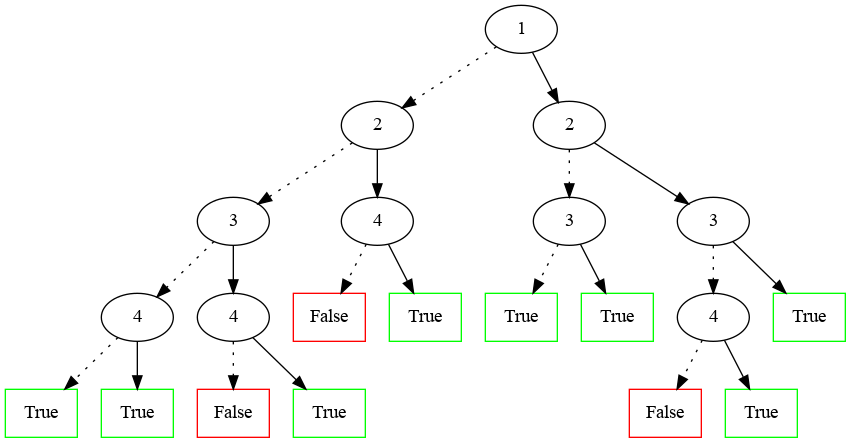
\includegraphics[scale=0.3]{../Images/arbre_compresse.png}
\caption{ZDD construit sur le grand entier [25899]}
\end{figure}

L'algorithme de compression que nous avons écrit nous semble alors fonctionner conformément aux attentes.

\section{Compression avec historique stocké dans une structure arborescente}

\section{Analyse de complexité}


\section{Étude expérimentale}

\end{document}